\documentclass{beamer}

%% TODO: Network algorithms for this class
% - detect articulation nodes
% - Minimum Spanning Tree -- OK!
% - Djisktra
% - Union find

%% Current Algorithms
% -  

%%% Algorithms: What do they do, what are they useful for, how to implement them.



\usepackage{amssymb,amsmath}
\usepackage{graphicx}
\usepackage{url}
\usepackage{color}
\usepackage{relsize}		% For \smaller
\usepackage{url}			% For \url
\usepackage{epstopdf}	% Included EPS files automatically converted to PDF to include with pdflatex
\usepackage{pagenote}[continuous,page]

%For MindMaps
% \usepackage{tikz}%
% \usetikzlibrary{mindmap,trees,arrows}%

%%% Color Definitions %%%%%%%%%%%%%%%%%%%%%%%%%%%%%%%%%%%%%%%%%%%%%%%%%%%%%%%%%
%\definecolor{bordercol}{RGB}{40,40,40}
%\definecolor{headercol1}{RGB}{186,215,230}
%\definecolor{headercol2}{RGB}{80,80,80}
%\definecolor{headerfontcol}{RGB}{0,0,0}
%\definecolor{boxcolor}{RGB}{186,215,230}

%%% Save space in lists. Use this after the opening of the list %%%%%%%%%%%%%%%%
%\newcommand{\compresslist}{
%	\setlength{\itemsep}{1pt}
%	\setlength{\parskip}{0pt}
%	\setlength{\parsep}{0pt}
%}

%\setbeameroption{show notes on top}

% You should run 'pdflatex' TWICE, because of TOC issues.

% Rename this file.  A common temptation for first-time slide makers
% is to name it something like ``my_talk.tex'' or
% ``john_doe_talk.tex'' or even ``discrete_math_seminar_talk.tex''.
% You really won't like any of these titles the second time you give a
% talk.  Try naming your tex file something more descriptive, like
% ``riemann_hypothesis_short_proof_talk.tex''.  Even better (in case
% you recycle 99% of a talk, but still want to change a little, and
% retain copies of each), how about
% ``riemann_hypothesis_short_proof_MIT-Colloquium.2000-01-01.tex''?

\mode<presentation>
{
  % A tip: pick a theme you like first, and THEN modify the color theme, and then add math content.
  % Warsaw is the theme selected by default in Beamer's installation sample files.

  %%%%%%%%%%%%%%%%%%%%%%%%%%%% THEME
  %\usetheme{Madrid}		% No subsection
  \usetheme{AnnArbor}  % Subsection on top, no color


  %\usetheme{Antibes}
  %\usetheme{Bergen}
  %\usetheme{Berkeley}		% bem bacana - menu esquerdo
  %\usetheme{Berlin}
  %\usetheme{Boadilla}
  %\usetheme{boxes}
  %\usetheme{CambridgeUS}		% bem bacana - menu superior
  %\usetheme{Copenhagen}
  %\usetheme{Darmstadt}
  %\usetheme{default}
  %\usetheme{Dresden}
  %\usetheme{Frankfurt}
  %\usetheme{Goettingen}
  %\usetheme{Hannover}		% bem bacana - menu esquerdo
  %\usetheme{Ilmenau}
  %\usetheme{JuanLesPins}
  %\usetheme{Luebeck}
  %\usetheme{Malmoe}
  %\usetheme{Marburg}		% bem bacana - menu direito
  %\usetheme{Montpellier}
  %\usetheme{PaloAlto}		% bem bacana - menu esquerdo
  %\usetheme{Pittsburgh}
  %\usetheme{Rochester}		%bacana
  %\usetheme{Singapore}
  %\usetheme{Szeged}
  %\usetheme{Warsaw}

  %%%%%%%%%%%%%%%%%%%%%%%%%%%% COLOR THEME
  %\usecolortheme{default}		% branco, azul clarinho
  \usecolortheme{crane}		% Very yellow (ok)

  %\usecolortheme{albatross}		% azul escuro, massa
  %\usecolortheme{beetle}		% cinza, menu azul
  %\usecolortheme{dolphin}		% azul e branco, legal
  %\usecolortheme{dove}			% cinza e branco, feio
  %\usecolortheme{fly}			% todo cinza, horrível
  %\usecolortheme{lily}			% parece o default
  %\usecolortheme{orchid}		% azul e branco, ok
  %\usecolortheme{rose}			% branco e violeta-claro, bonito
  %\usecolortheme{seagull}		% cinza, feio
  %\usecolortheme{seahorse}		% nhé, meio feio
  %\usecolortheme{sidebartab}		% Azul, branco, destaque na tab, interessante
  %\usecolortheme{structure}		% bichado
  %\usecolortheme{whale}		% Azul e branco, bem bonito

  %%%%%%%%%%%%%%%%%%%%%%%%%%%% OUTER THEME
  \useoutertheme{default}
  %\useoutertheme{infolines}
  %\useoutertheme{miniframes}
  %\useoutertheme{shadow}
  %\useoutertheme{sidebar}
  %\useoutertheme{smoothbars}
  %\useoutertheme{smoothtree}
  %\useoutertheme{split}
  %\useoutertheme{tree}

  %%%%%%%%%%%%%%%%%%%%%%%%%%%% INNER THEME
  \useinnertheme{circles}
  %\useinnertheme{default}
  %\useinnertheme{inmargin}
  %\useinnertheme{rectangles}
  %\useinnertheme{rounded}

  %%%%%%%%%%%%%%%%%%%%%%%%%%%%%%%%%%%

  \setbeamercovered{invisible} % or whatever (possibly just delete it)
  % To change behavior of \uncover from graying out to totally
  % invisible, can change \setbeamercovered to invisible instead of
  % transparent. apparently there are also 'dynamic' modes that make
  % the amount of graying depend on how long it'll take until the
  % thing is uncovered.

}


% Get rid of nav bar
\beamertemplatenavigationsymbolsempty

% Use short top
%\usepackage[headheight=12pt,footheight=12pt]{beamerthemeboxes}
%\addheadboxtemplate{\color{black}}{
%\hskip0.5cm
%\color{white}
%\insertshortauthor \ \ \ \
%\insertframenumber \ \ \ \ \ \ \
%\insertsection \ \ \ \ \ \ \ \ \ \ \ \ \ \ \ \ \  \insertsubsection
%\hskip0.5cm}
%\addheadboxtemplate{\color{black}}{
%\color{white}
%\ \ \ \
%\insertsection
%}
%\addheadboxtemplate{\color{black}}{
%\color{white}
%\ \ \ \
%\insertsubsection
%}

% Insert frame number at bottom of the page.
% \usefoottemplate{\hfil\tiny{\color{black!90}\insertframenumber}}

%% makes the ppagenote command for figure references at the end.

\usepackage[english]{babel}
%qq\usepackage[latin1]{inputenc}
\usepackage{CJKutf8}
\usepackage{subfigure}

\usepackage{times}
\usepackage[T1]{fontenc}

\makepagenote
\renewcommand{\notenumintext}[1]{}
\newcommand{\ppagenote}[1]{\pagenote[Page \insertframenumber]{#1}}

\title[Programming Challenges]{GB20602 - Programming Challenges}
\author[Claus Aranha]{Claus Aranha\\{\footnotesize caranha@cs.tsukuba.ac.jp}}
\institute[U. Tsukuba]{University of Tsukuba, Department of Computer Sciences}


\title[]{Software Science Seminar}
\subtitle[]{Week 8 - Graph Algorithms}
\author[Claus Aranha]{Claus Aranha\\{\footnotesize caranha\@@cs.tsukuba.ac.jp}}
\institute{College of Information Sciences}
\date{2015-06-15\\{\tiny Last updated \today}}

\begin{document}
\section{Introduction}
\subsection{Introduction}

\begin{frame}
\maketitle
\end{frame}

\begin{frame}
  \frametitle{Outline}
  \begin{itemize}
  \item \emph{Part I:} Graph properties (node properties, cicles, etc)
  \item \emph{Part II:} Graph algorithms (spanning tree, flow)
  \end{itemize}
\end{frame}

\section{Graph Properties}
\subsection{Graph Theory}

\begin{frame}
  \begin{center}
    Part I: Graph Properties
  \end{center}
\end{frame}

\begin{frame}
  \frametitle{Degree Properties}
  {\small
  \begin{block}{Vertex Degrees}
    \begin{itemize}
    \item The \structure{degree} of a vertex is the total number of edges
      connected to it.
    \item For \emph{Undirected Graphs}: Total Degrees = 2*total edges. Why?
    \item For \emph{Directed Graphs}: We count in-degrees and
      out-degrees; Total in-degrees = total out-degrees;
    \end{itemize}
  \end{block}}
  \begin{center}
    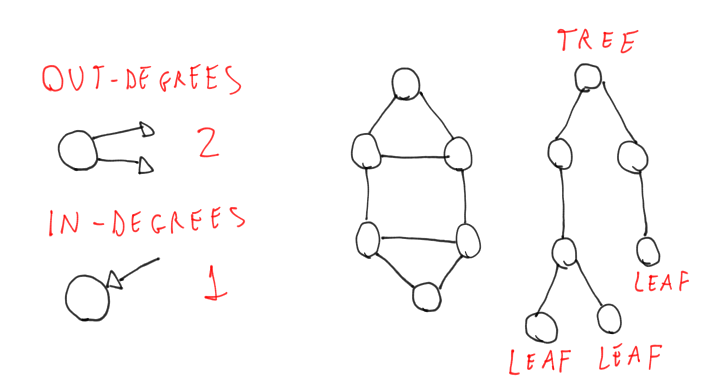
\includegraphics[width=0.7\textwidth]{img/degrees1}
  \end{center}
\end{frame}

\begin{frame}
  \frametitle{Degree Properties}
  {\small
  \begin{block}{Trees}
    \begin{itemize}
    \item Trees are undirected graphs with no cycles.
    \item \structure{Leaf} nodes are nodes with degree 1;
    \item Every n-vertex tree contains 1-n edges.
    \item \structure{Rooted Trees} are directed graphs where every
      node except the root has in-degree 1. Leaves have out-degree 0.
    \end{itemize}
  \end{block}}
  \begin{center}
    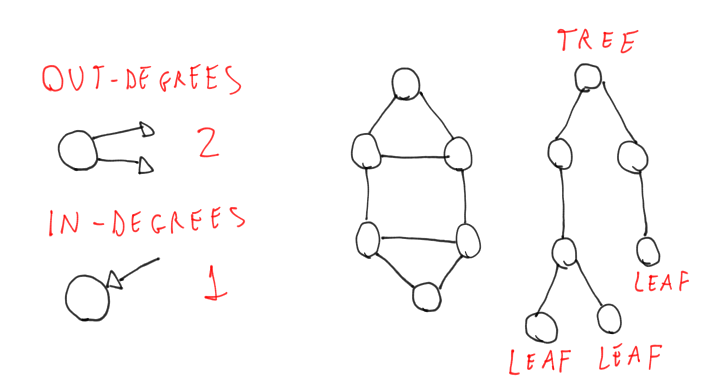
\includegraphics[width=0.7\textwidth]{img/degrees1}
  \end{center}
\end{frame}




\begin{frame}
  \frametitle{Degree Properties}
  {\small
  \begin{block}{Spanning Trees}
    \begin{itemize}
    \item The spanning tree of graph G(V,E) is the subset G(V,E') that
      forms a tree in G.
    \item Any connected graph has a spanning tree.
    \item \structure{The Minimum Spanning Tree} is a important
      characteristic of weighted graphs.
    \end{itemize}
  \end{block}}

  \begin{center}
    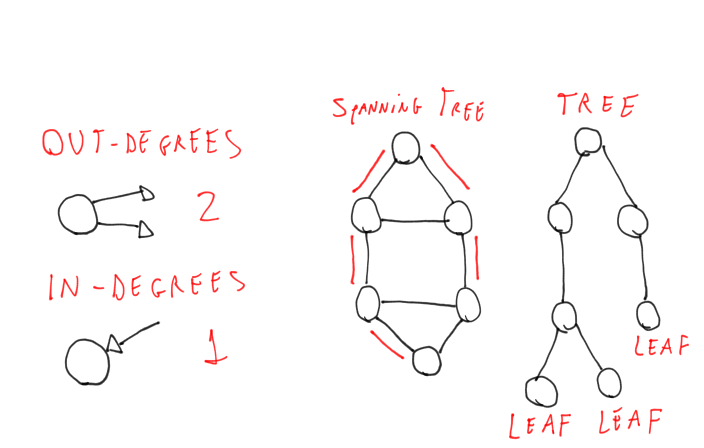
\includegraphics[height=0.45\textheight]{img/degrees2}
  \end{center}
\end{frame}

\subsection{Connectivity}

\begin{frame}
  \frametitle{Connectivity}
  \begin{block}{Definitions of Connectivity}
    {\smaller
    \begin{itemize}
    \item \structure{Connected Graph}: There is a path between any pair of vertices;
    \item The existence of a spanning trees guarantees connectivity;
    \end{itemize}
    }
  \end{block}
  
  \begin{center}
    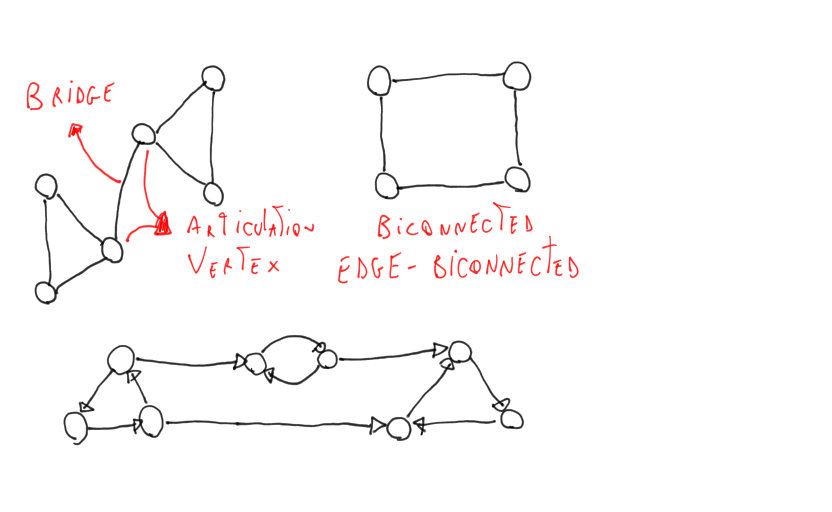
\includegraphics[width=0.7\textwidth]{img/biconnected}
  \end{center}
\end{frame}

\begin{frame}
  \frametitle{Connectivity}
  \begin{block}{Definitions of Connectivity}
    {\smaller
      \begin{itemize}
      \item \structure{Vertex Connectivity}: number of vertices that
        need to be deleted to ``disconnect'' the graph;
      \item If Vertex connectivity is 1, we have an
        \structure{articulation vertex}
      \item If there are no articulation vertices, the graph is
        \structure{biconnected}
      \item Finding by brute force: remove each vertex, and test for
        connectivity;
    \end{itemize}}
  \end{block}
  
  \begin{center}
    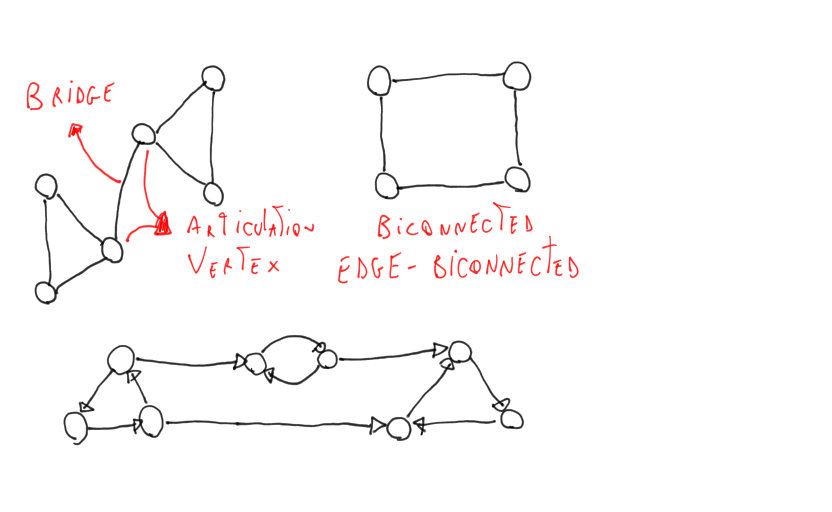
\includegraphics[width=0.7\textwidth]{img/biconnected}
  \end{center}
\end{frame}

\subsection{Cycles}

\begin{frame}
  \frametitle{Cycles}
  \begin{center}
    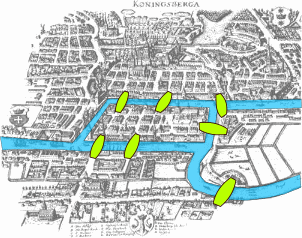
\includegraphics[width=0.4\textwidth]{img/eulerian}
  \end{center}
  {\small
  \begin{block}{Eulerian Cycle}
    \begin{itemize}
    \item Each edge of the graph is visited exactly once.
    \item Connected, undirected graphs are eulerian if every vertex
      has even degree. Why?
    \item Directed graphs are Eulerian if in-degree = out-degree for
      all vertices;
    \item How can we find an Eulerian cycle?
    \end{itemize}
  \end{block}}
\end{frame}

\begin{frame}
  \frametitle{Cycles}
  \begin{center}
    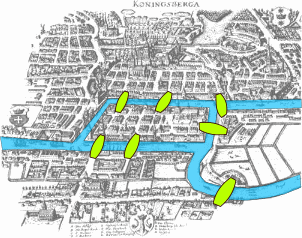
\includegraphics[width=0.5\textwidth]{img/eulerian}
  \end{center}
  {\small
    \begin{block}{Hamiltonian Cycles}
      \begin{itemize}
      \item Each vertex of the graph is visited exactly once;
      \item Not so easy to find a solution as the Eulerian cycle;
      \end{itemize}
    \end{block}
  }
\end{frame}

\begin{frame}
  \frametitle{Cycles}
  \begin{center}
    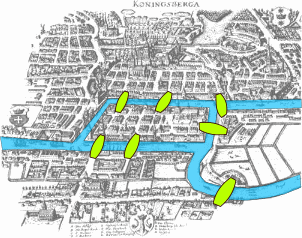
\includegraphics[width=0.5\textwidth]{img/eulerian}
  \end{center}
\end{frame}

\section{Algorithms}
\subsection{Minimum Spanning Tree}

\begin{frame}
  \begin{center}
    Part II: Graph Algorithms
  \end{center}
\end{frame}

\begin{frame}
  \frametitle{Minimum Spanning Trees}
  \begin{block}{}
    \begin{itemize}
    \item \structure{Spanning Tree}: A subset tree of a graph that includes all nodes.
    \item \structure{Minimum Spanning Tree}: The spanning Tree that has minimal weight.
    \end{itemize}
  \end{block}
  \begin{center}
    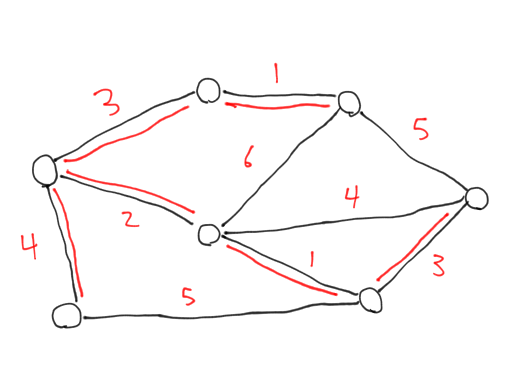
\includegraphics[width=0.7\textwidth]{img/minspantree}
  \end{center}
\end{frame}

\begin{frame}[fragile,singleslide]
  \frametitle{Minimum Spanning Tree}
  \begin{block}{Prim's Algorithm to find the MST}
    {\smaller
    Greedy algorithm:
\begin{verbatim}
1- Sort all edges by weight. 
2- Add the smallest edge to MST.
3- Sort edges that are connected to the MST.
4- Add the smallest edge with one new node to MST.
5- Go to 3.
\end{verbatim}}
  \end{block}
  \begin{center}
    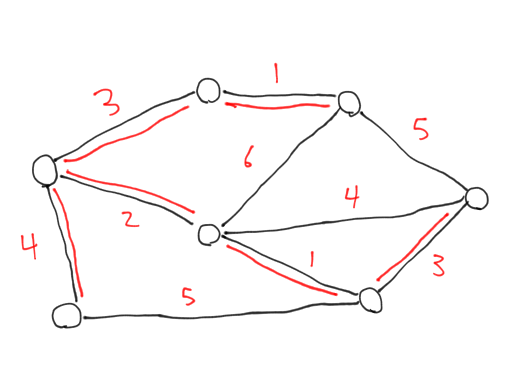
\includegraphics[width=0.6\textwidth]{img/minspantree}
  \end{center}
\end{frame}

\begin{frame}
  \frametitle{Minimum Spanning Tree}
  \begin{center}
    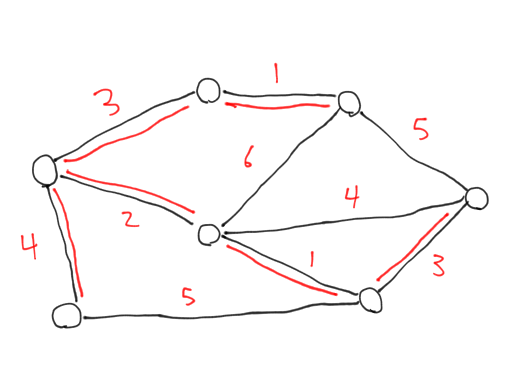
\includegraphics[width=0.6\textwidth]{img/minspantree}
  \end{center}
  \begin{itemize}
  \item Maximum Spanning Tree: -1*weight;
  \item Multiplication Spanning Tree: log(weight);
  \end{itemize}
\end{frame}

\begin{frame}[singleslide,fragile]
  \frametitle{Articulated Vertex Problem}
  An algorithm to find an articulated vertex in a graph was 
  discussed in the last class. 
  \bigskip
  {\smaller
\begin{verbatim}
1- Create a spanning tree using DFS
2- Rank each node by search order.
3- Back edges are not part of the DFS

4- Give a second rank to each node, based on the 
   highest rank they can reach using a back node.

5- Nodes where all children have second rank 
   smaller than themselves are articulation nodes.

\end{verbatim}
  }
\end{frame}

\begin{frame}
  \frametitle{Shortest Path}
  \begin{block}{Djikstra Algorithm}
    \begin{itemize}
    \item Very similar to Prim: What is the difference?
    \item When does this algorithm encounter problems?
    \end{itemize}
  \end{block}
  
  \begin{center}
    \includegraphics<1>[width=0.6\textwidth]{img/djikstra1}
    \includegraphics<2>[width=0.4\textwidth]{img/djikstra2}
  \end{center}
\end{frame}

\begin{frame}[fragile,singleslide]
  \frametitle{All-Pairs Shortest Path}
  {\smaller
  \begin{block}{Floyd's Algorithm (A bit similar to DP)}
    \begin{itemize}
    \item We want to find the shortest distance from all nodes to all nodes;
    \item Needs an adjacency Matrix (code/idea is simple);
    \item Iterate over nodes usable in the path;
    \item usable to test for unreachable nodes (infinite distance at the end);
    \end{itemize}
  \end{block}
\begin{verbatim}

weight[][] is adjacency matrix, unconnected nodes are INF

for (k = 1 to n-vertices):
  for (i = 1 to n-vertices):
    for (j = 1 to n-vertices):
      path_k = weight[i][k]+weight[k][j]
      if path_k < weight[i][j]:
        weight[i][j] = path_k
\end{verbatim}
}
\end{frame}

\begin{frame}
  \frametitle{Union-Find Problem}
  {\small
  Union-find is an algorithms that creates a structure to
  \structure{construct a set} from disjoint nodes. It has two main
  functions:

  \smallskip

  \begin{itemize}
    \item Union(Set A, Set B) - Merges set A with set B
    \item Find(Node A) - finds what set node A belongs to.
  \end{itemize}

  \bigskip

  In the beginning, all nodes belong to a set containing only
  themselves. Progressive application of Union will create the
  different sets using double linked lists.
  }
\end{frame}

%% TODO: Re-write network flow more carefully
\begin{frame}
  \frametitle{Network Flow}
  \begin{itemize}
  \item How much flow can we get from node $A$ to node $B$ at once?
  \item Ford-Fulkerson ``Augmenting Path'' algorithm:
  \item Basic idea: Do a BFS, remove ``flow'' from weight, repeat the BFS with new weights.
  \end{itemize}
  \begin{center}
    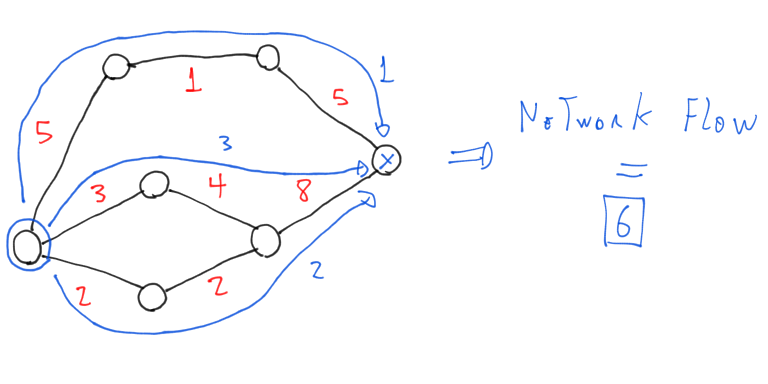
\includegraphics[width=0.8\textwidth]{img/netflow}
  \end{center}

\end{frame}

\section{Problems}
\subsection{Problems}
\begin{frame}
  \frametitle{This Week's Problems}
  \begin{itemize}
    \item Freckles
    \item Fire Station
    \item Tourist Guide
    \item War
  \end{itemize}


\end{frame}

\end{document}
